\documentclass[a4paper]{article}

\usepackage{graphicx}
\usepackage{hyperref}
\graphicspath{{../images/}}

\title{Analysis of Cryptographic Algorithms}
% Name of the project team and all members (full names and email addresses).

\author{
  Asad Raza\\
  \texttt{ar06246@st.habib.edu.pk}
  \and
  Batool Ahmed\\
  \texttt{ba06180@st.habib.edu.pk}
  \and 
  Haania Siddiqui\\
  \texttt{hs06188@st.habib.edu.pk}
  \and
  Shamsa Hafeez\\
  \texttt{sd06162@st.habib.edu.pk}
  \and 
  Team: random-path \\
}



\maketitle
\begin{document}

\section{Description} %A short description of the chosen problem (about 300 - 500 words) with one or two figures (for illustration).

Cryptography means "the study of secret"$^{[2]}$. Nowadays, the term "cryptography" is usually associated with encryption $^{[2]}$.Encryption is "the process of converting human-readable plain text to incomprehensible text, also known as cipher text." $^{[4]}$ Thus, data encryption is "a way of translating data from plain text (unencrypted) to cipher text (encrypted)" $^{[5]}$. The methods via which given data is transformed into ciphertext are encryption algorithms $^{[4]}$. "Encryption algorithms use encryption key in order to alter the data in a predictable way, so that even though the encrypted data will appear random, it can be turned back into plain text by using the decryption key." $^{[4]}$. \\
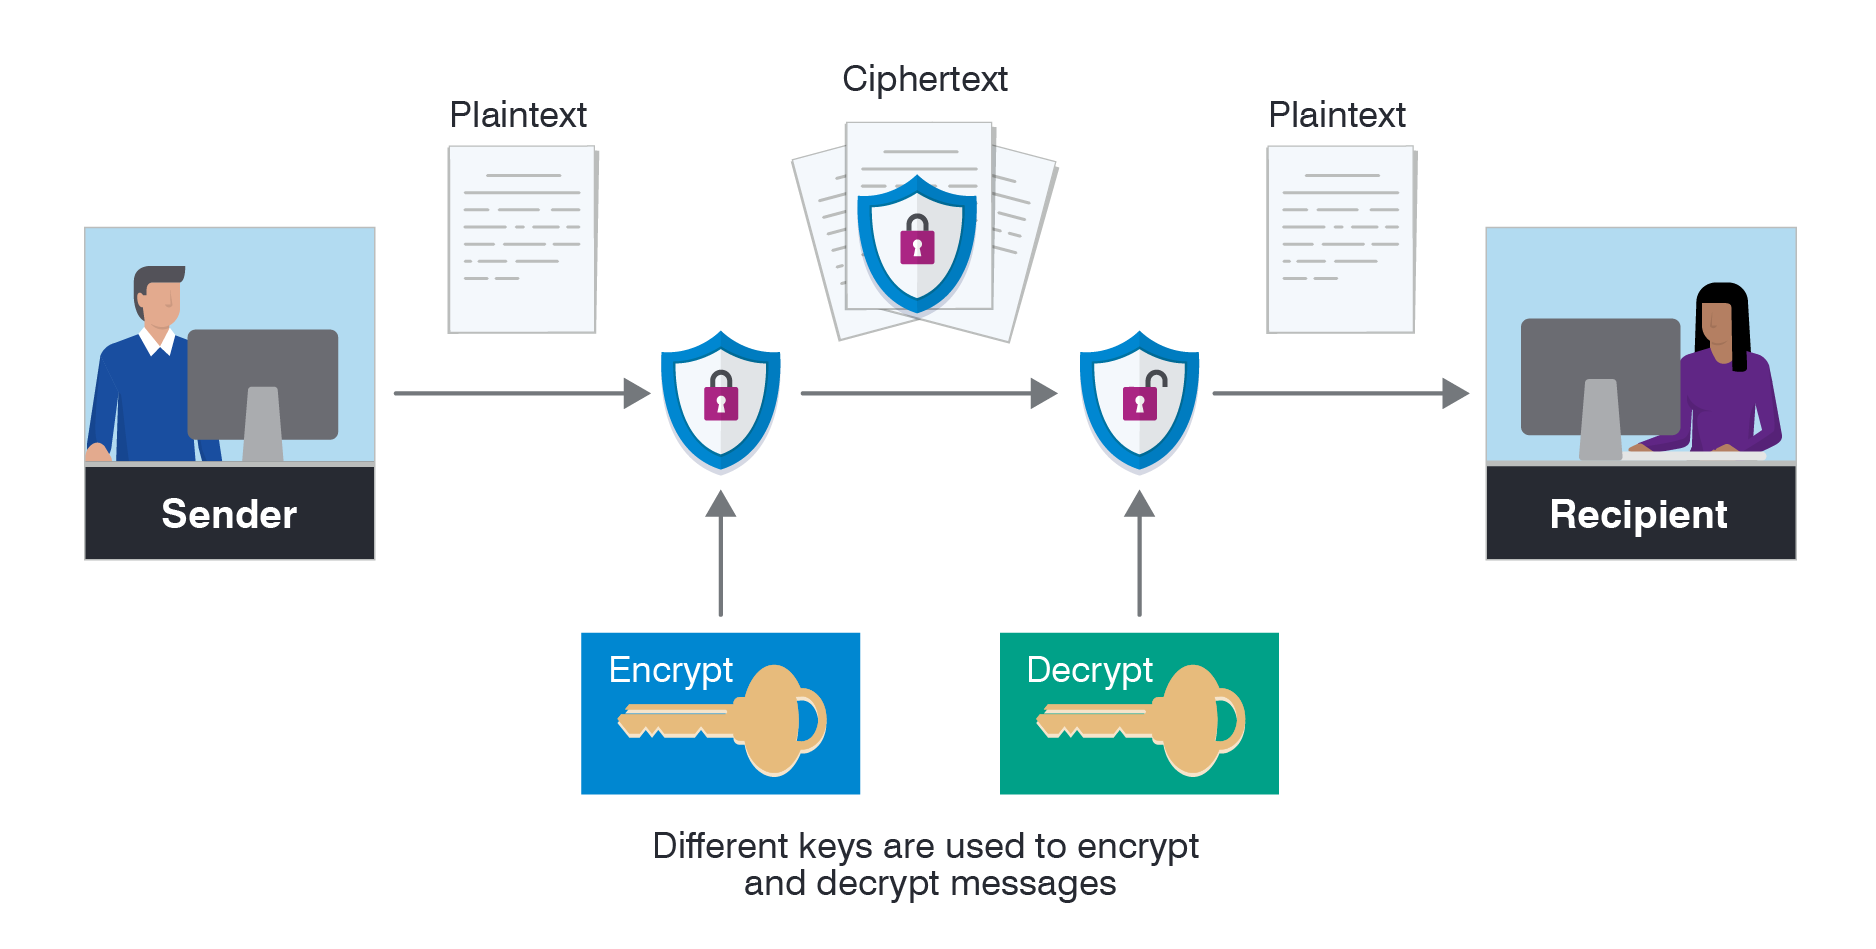
\includegraphics[width=10cm]{images/what-is-encryption.png}\\
Encryption algorithms provide security against unauthorized attacks $^{[1]}$. In order to prevent security breach, not only must these algorithms ensure security, they must also have fast performance because it is a common practice to embed encryption algorithms in applications that require fast performance $^{[1]}$. For example: e-commerce, banking, and online transaction processing applications$^{[1]}$. \\

In this project, we aim to perform algorithmic analysis on some of the cryptographic Algorithms. Note that this performance analysis would not compare the algorithms based on the level of security that it provides, rather it will only compare their performance based on run time. To ensure the accuracy of the comparison, all algorithms will be tested on a single system using a particular language.$^{[1]}$


\newpage 
\section{Algorithms/design techniques} %Algorithms/design techniques to be explored and implemented.
Following are some of the encryption algorithms that would be included in analysis: \\
1. Data Encryption Standard (DES) algorithm\\ 
2. Rivest-Shamir-Adelman (RSA) Algorithm \\
3. Blowfish Algorithm \\


\section{References}
$[1]$ \url{https://ieeexplore.ieee.org/abstract/document/1598556}\\
$[2]$ \url{https://www.cse.wustl.edu/~jain/cse567-06/ftp/encryption_perf/}\\
$[3]$ \url{https://www.proofpoint.com/us/threat-reference/encryption}\\
$[4]$ \url{https://www.cloudflare.com/learning/ssl/what-is-encryption/}\\
$[5]$ \url{https://www.ibm.com/topics/encryption}\\ 



\end{document}
